\documentclass{report}
\usepackage[utf8]{inputenc}
\usepackage[brazil]{babel}
\usepackage{graphicx}
\usepackage{float}

\title{Programação para Iniciantes \\ \large 1ª Edição}
\author{Ralph dos Santos Souza}
\date{\today}

\begin{document}

\maketitle

\tableofcontents

\chapter*{Introdução}
\addcontentsline{toc}{chapter}{Introdução}
\begin{center}
    Antes de começarmos permitam-me dar-lhes as boas vindas ao Programação para Iniciantes. Este livro tem como objetivo
    apresentar os conhecimentos básicos no mundo da Tecnologia da Informação para àqueles que nunca antes se aventuraram por aqui
    e que agora buscam trilhar este caminho.\\
    \vspace{12pt}
    Este livro surgiu da minha própria experiência, no início da minha jornada, quando comecei a entender alguns pontos e conceitos
    importantes da área, coisas que uma pessoa que nunca teve qualquer contato com a área jamais teria como conhecer. 
    É claro que assim como eu consegui entender os mesmos qualquer pessoa conseguiria mas, por quê procurar informações distintas 
    em lugares distintos se poderemos fazer o mesmo através desta obra?\\
    \vspace{12pt}
    Aqui nós iremos entender o que é uma \textbf{stack}, qual a melhor aplicação práticas para certas linguagens, o que são \textbf{frameworks}, 
    quais são os papéis desempenhados pelo \textbf{backend} e pelo \textbf{frontend}, o que é um programador \textbf{fullstack}, o que faz
    um \textbf{QA (Quality Assurance)}, qual o papel do \textbf{DevOps}, qual o papel do \textbf{DBA (Database Analist)}, entre muitas outras
    coisas.\\
    \vspace{12pt}
    É claro que não iremos nos aprofundar em cada um desses pontos, afinal de contas cada um é um universo à parte, infinito em conhecimento 
    e informação. A proposta aqui é outra, é permitir que você, que busca ingressar nessa área, possa entender um pouco mais, de maneira
    prática e quem sabe divertida, sobre os desafios ocultos do TI.
\end{center}

\chapter*{Agradecimentos}
\addcontentsline{toc}{chapter}{Agradecimentos}
\begin{center}
    
\end{center}

\chapter{Algoritmo, Automação, Programa de Computador}
    Existem questões que precisaremos abordar durante nossa jornada pelo mundo da programação, mesmo que este seja um guia básico
    para quem está começando sua jornada ele trará diversas informações sobre processos, conceitos, paradignmas, entre outras coisas. Tudo que veremos
    aqui fará parte do nosso dia a dia. Neste capítulo iremos falar um pouco mais sobre o que são \textbf{Algoritmos}, \textbf{Automação} e 
    \textbf{Programa de Computador}. Primeiramente iremos falar sobre a definição de cada um desses tópicos e posteriormente entraremos um 
    pouco mais a fundo nos conceitos.\\
    \vspace{12pt}
    \begin{enumerate}
        \item \textbf{Algoritmo}
    \end{enumerate}
    \textbf{Definição:} Algoritmo é uma sequência finita de instruções para se resolver um problema. Quando ouvimos a palavra \textbf{Algoritmo} 
    nossa mente tende automáticamente a pensar em programação certo? Porém, \textbf{Algoritmos} podem ser aplicados à diversas áreas, 
    tanto no âmbito profissional quanto no âmbito pessoal, vejamos o exemplo a seguir:\\
    \vspace{12pt}
    \textbf{Exemplo 1: Desenvolvimento de Software}
    \begin{figure}[H]
        \centering
        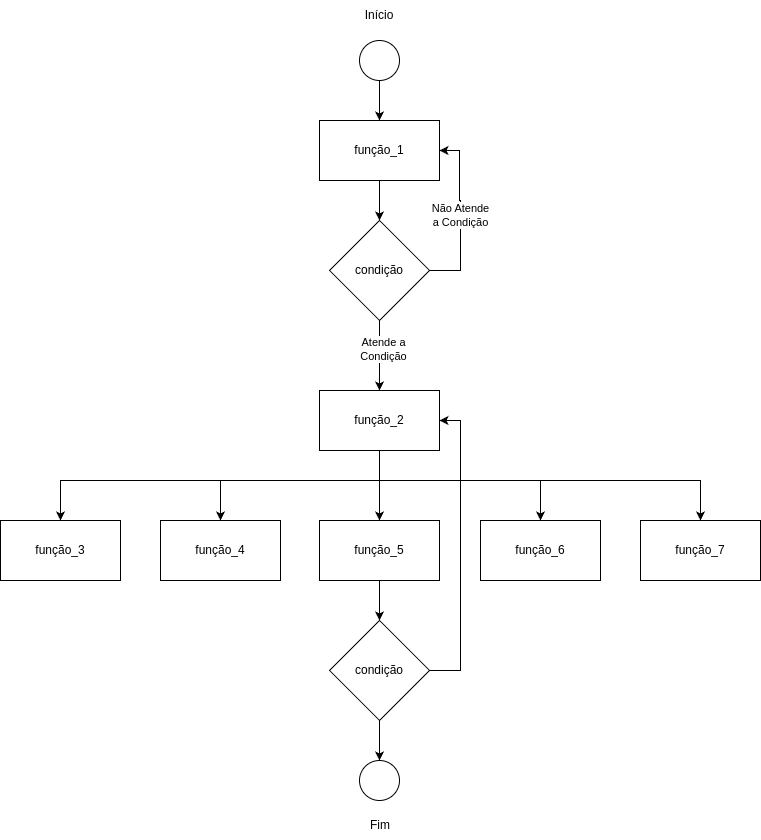
\includegraphics[width=1.0\textwidth]{img/software.drawio.png}
        \caption{Exemplo 1}
        \label{fig:Exemplo 1}
    \end{figure}
    \textbf{Exemplo 2: Dia a dia}
    \begin{figure}[H]
        \centering
        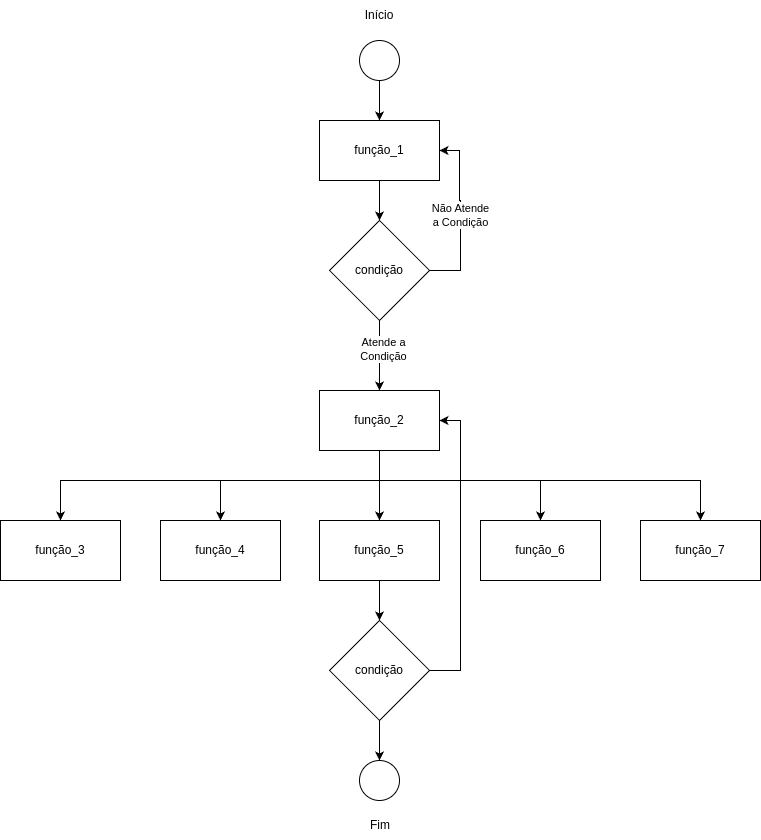
\includegraphics[width=0.5\textwidth]{img/software.drawio.png}
        \caption{Exemplo 2}
        \label{fig:Exemplo 2}
    \end{figure}
\chapter{}

\end{document}